\subsection{Gaussian processes}
\label{sec:chol}

Many uncertainty quantification applications replace an
expensive model, such as a discretised partial differential equation, with a
cheap surrogate.  This is done so that during a Markov chain Monte Carlo
procedure, likelihood evaluations are cheap.  There are a plethora of different
surrogate choices and strategies for choosing which is appropriate for a
particular application.  Gaussian processes are a common choice, and we explore
their scaling on the KNL architecture here.\todo{citations motherclucker, do you have them?}

Gaussian processes are a probabilistic model for generating random fields
characterised by a mean $\mu$ function and a covariance function $c$,
\begin{equation}
  f(x) \sim \mathcal{N}(\mu(x), c(x, x')).
\end{equation}

They have the property that evaluation of the field at some finite set of
points $(x_1, \ldots, x_n)$ yields a multivariate normal vector with a known
mean vector and symmetric and positive-definite covariance matrix
\begin{equation}
  \begin{pmatrix}
    f(x_1) \\
    \hdots \\
    f(x_n)
  \end{pmatrix}
  \sim \mathcal{N}(\mu, \Sigma).
\end{equation}
Thus, laying down a grid of points at which we wish to model the field yields
the usual Gaussian probability distribution function we are familiar with,
\begin{equation}
  p(x) \propto |\Sigma|^{-1/2} \exp(-\frac12 x^\top \Sigma^{-1} x).
\end{equation}
Notice that evaluation of this probability density function necessitates a
linear solve $\Sigma u = x$.  Since $\Sigma$ is symmetric and positive-definite
a Cholesky factorisation is required.  Iterative approaches exist too, but we
concentrate on the direct approach for this work.  It is also worth noting that the
covariance function typically takes an exponential form
\begin{equation}
  c(x, x') = \sigma^2 \exp(-\frac12 \| x - x' \|^2 / l^2)
\end{equation}
and so the resulting covariance matrix
\begin{equation}
  \Sigma_{ij} = c(x_i, x_j)
\end{equation}
is full and dense.  The covariance function can also contain
unknown hyperparameters
that need to be inferred, for example, a hierarchical
Bayesian setting.  The usual approach to evaluate the
probability density function is: 
\begin{enumerate}
  \item Compute $L$ such that $\Sigma = LL^\top$.
  \item Solve $\Sigma u = x$ using (1).
  \item Compute the inner-product $x^\top u$.
  \item Divide by the square root of the determinant of $\Sigma$.
  \item Return $p$
  \item Go to (1) for the next state in the Markov chain.
\end{enumerate}

QUESO was used to manage the Gaussian process and Markov chain infrastructure.
The bulk of the computational cost lies inside the likelihood function which
necessitates the evaluation of the Gaussian probability density function.
Extensive use of Intel's MKL was used for both the Cholesky factorisation,
subsequent linear solve, and determinant calculation.

Figure~\ref{fig:gp} shows timings of a Gaussian process likelihood evaluation
as a function of number of OpenMP threads.  The timings only include the
assembly and the factorisation, since these two procedures are the most
expensive at each iteration of a Markov chain Monte Carlo procedure.  The
assembly was parallelized with the usual OpenMP preprocessor directives, and
the factorization was executed by Intel's MKL.  Two cases were run, one
entirely in MCDRAM and the other entirely in DDR4.  Timings for both of these
show that for problems that are not memory-bandwith limited, MCDRAM does not
offer a significant payoff.

%
% Can you say something about strong-weak scaling?  this looks like a strong
% scaling analysis, can you detail more on the speedup?
%
% DM -- happy to do weak, concerned about the page limit given csim still needs
% to add his stuff, though.  let me know what you think is best.
\begin{figure}
  \begin{center}
    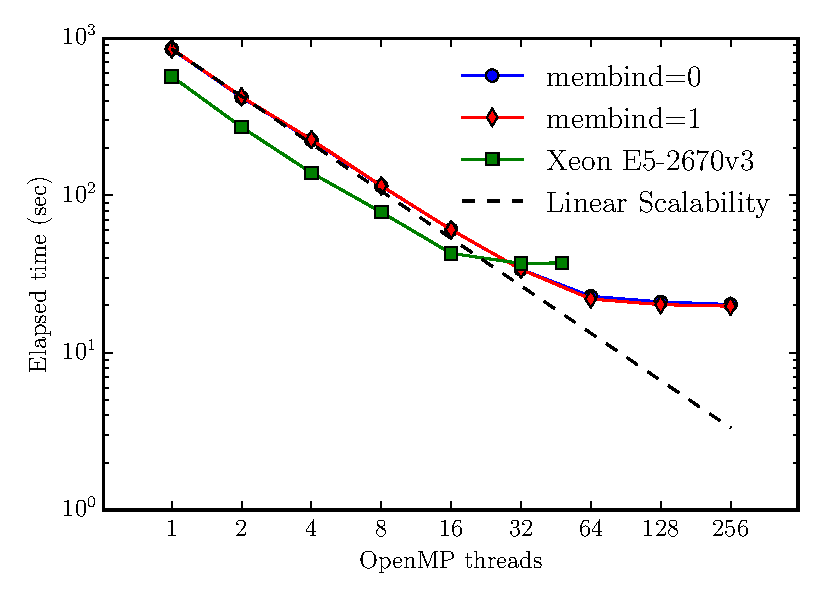
\includegraphics[width=0.45\textwidth]{gp_membind_scaling_collapse.pdf}
    \caption{Strong scaling of time taken to execute both a Gaussian process
    assembly and factorization.  The red line shows the case where the problem
    was allocated entirely in MCDRAM.  The blue line shows the case where the
    problem was allocated entirely in DDR4.}
    \label{fig:gp}
  \end{center}
\end{figure}
